\documentclass{beamer}
\usepackage[norsk]{babel}
\usepackage[utf8]{inputenx}
\usepackage[stickyper,obeyall,locale=DE,dp=4]{siunitx}
\usetheme{Pittsburgh}
\setbeamercolor{normal text}{bg=red!7}
\setbeamertemplate{footline}{\insertpagenumber}
\usepackage{xmpmulti,amsmath,amssymb,graphicx,mflogo}
\DeclareGraphicsRule{*}{mps}{*}{}
\graphicspath{{./metapostpropagandafiles/}}
\newcommand{\myem}[1]{\texttt{#1}}
\title{Wide--range \MP\ tutorial}
\author{
  Luís Nobre Gonçalves \\
  (\href{mailto:lnobreg@gmail.com}{\underline{L. Nobre G.}})
}
\date{\today}
\begin{document}
\frame{
  \titlepage
  \begin{abstract}
    Sort of workshop about \TeX--things, focusing on the \MP\ language.
  \end{abstract}
}

\frame{
  \frametitle{The Church of Free Software}
  Pope: \href{http://stallman.org/}{\underline{Richard Stallman}}.
}

\frame{
  \frametitle{Evil}
  {\LARGE WYSIWYG}
  \pause

  What you get is what you \textcolor{red}{don't} see
}

\frame{
  \frametitle{Freedom}
  You choose what you get \pause

  but

  you only get it at the end of a long path.
}

\frame{\tableofcontents}

\section{Introduction}
 
\subsection{A bit of history}

\frame{
  \frametitle{A bit of history}
  \href{http://news.stanford.edu/news/2011/june/knuth-engineering-hero-060111.html}{\underline{Donald Knuth -- \textit{The Art of Computer Programming}}}
  \begin{itemize}
  \item Volume1, 1969, hot metal
  \item Volume2, $2^{\mathrm{\underline{nd}}}$ ed., 1977, photographic
  \item \TeX, v1, 1978, $\mathrm{v}\longrightarrow\pi$
  \item \MF, v1, 1979, $\mathrm{v}\longrightarrow e$ --- \textrm{affine}
  \item AMS, 1983
  \item APS, AIP, OSA, AAS, Springer-Verlag
  \item \MP, 1994, John Hobby
  \end{itemize}  
  \pause
  \MP\ is the realm of graphic \textcolor{green}{parameterization}.
}

\subsection{What is \MP ?}

\frame{
  \frametitle{Main features of \MP}
  \begin{itemize}
  \item It is easy to express geometry as \MP\ code
  \item \MP\ outputs \myem{postscript}, SVG or PNG
    \begin{quote}
      \myem{outputformat := \dq svg\dq;}
    \end{quote}
  \item Very good control of 2D B\'{e}zier splines
  \item Special 2D operators
  \item Many operators work the same way in 1, 2, 3 or 4D
  \item Linear equations
  \item May include \LaTeX
  \item May be included in \LaTeX
  \end{itemize}  
}

\subsection{Main reason to use \MP}

\frame{
  \frametitle{Use \MP\ because}
  \MP\ helps the user to experiment different
  diagram layouts without changing specified 
  \textcolor{green}{geometric relationships} among diagram elements.
}

\section{For Almost Absolute Beginners}

\frame{
  \frametitle{For Almost Absolute Beginners}
  \begin{itemize}
    \item Availability
    \item Mathematically oriented
    \item Programmability/Scriptability
    \item Forced simplicity
    \item \textcolor{green}{Consistency}
  \end{itemize}
}  

\subsection{Availability}

\frame{
  \frametitle{Availability}
  \begin{itemize}
  \item \href{http://foundry.supelec.fr/gf/project/metapost}{\underline{Development site}}
  \item \href{http://www.ctan.org/}{\underline{CTAN}}
    \begin{itemize}
    \item \href{http://www.ctan.org/tex-archive/graphics/metapost/contrib/macros}{\underline{/graphics/metapost/contrib/macros}}
    \end{itemize}
    \pause
  \item \TeX\ Users Group
    \begin{itemize}
    \item \href{http://www.tug.org/texlive/}{\underline{\texttt{texlive}}}
    \end{itemize}
  \item \href{http://packages.debian.org/search?keywords=texlive&searchon=names&suite=stable&section=all}{\underline{Debian}}
    \begin{itemize}
    \item \href{http://packages.debian.org/squeeze/texlive-metapost}{\underline{\texttt{texlive-metapost}}}
    \item \href{http://packages.debian.org/squeeze/texlive-publishers}{\underline{\texttt{texlive-publishers}}} includes \href{https://authors.aps.org/revtex4/}{\underline{RevTeX}}
    \item \href{http://packages.debian.org/squeeze/latex-beamer}{\underline{\texttt{latex-beamer}}}
    \item \href{http://tug.org/tex4ht/}{\underline{\texttt{tex4ht}}}
    \end{itemize}
  \item ``The \LaTeX\ Companions''
  \end{itemize}
}

\subsection{Mathematically oriented}

\frame{
  \frametitle{Linear equations}
  \begin{center}
    \includegraphics[height=35mm]{intersection2D.1}
    \\
    \begin{itemize}
    \item Constraints may be expressed as linear equations
      \begin{quote}
        \myem{z5 = whatever[z1,z2];} \\
        \myem{z5 = whatever[z3,z4];}
      \end{quote}
    \item No need to explicitly assign calculations to unknowns
    \end{itemize}
  \end{center}
}

\frame{
  \frametitle{\myem{pair} doublets}
  \begin{itemize}
  \item \myem{pair} 
    \begin{tabular}[t]{cc}
      \myem{(\textit{x,y})}$\longrightarrow$ & \myem{(X,Y)} \\
      \myem{origin} & (0,0)
    \end{tabular}
  \item Coordinates
    \begin{quote}
      \myem{z[i] = (x[i],y[i]);}
     \end{quote}
  \end{itemize} 
}

\frame{
  \frametitle{\myem{color} triplets}
  \begin{itemize}
  \item \myem{color} 
    \begin{tabular}[t]{cc}
      \myem{(\textit{red,green,blue})}$\longrightarrow$ & \myem{(X,Y,Z)} \\
      \myem{black} & (0,0,0) \\
      \myem{red} & (1,0,0) \\
      \myem{green} & (0,1,0) \\
      \myem{blue} & (0,0,1) \\
      \myem{white} & (1,1,1) 
    \end{tabular}
  \end{itemize} 
}

\frame{
  \frametitle{\myem{cmykcolor} tetraplets}
  \begin{itemize}
  \item \myem{cmykcolor} 
      
    \myem{(\textit{cyan,magenta,yellow,black})}$\longrightarrow$\myem{(X,Y,Z,W)}
    (\href{http://en.wikipedia.org/wiki/Quaternions_and_spatial_rotation}{\underline{quaternions}},
    \href{http://en.wikipedia.org/wiki/Homogeneous_coordinates}{\underline{homogeneous coordinates}}, 4D splines, animation frames, straight line segments, etc.) 
  \end{itemize} 
}

\frame{
  \frametitle{Special operators}
  \begin{itemize}
  \item Pythagorean addition and subtraction
    \begin{quote}
      \myem{h = a ++ b +-+ c;} ($h=\sqrt{a^2+b^2-c^2}$)
    \end{quote}
    \pause
  \item Interval 0---1 ND operator s[,]
    \begin{quote}
      \begin{tabular}{lcl}
        \myem{0.5[(1,1),(3,5)]}         & $\longrightarrow$ & \myem{(2,3)} \\
        \myem{-0.5[(1,1,1),(3,5,7)]}    & $\longrightarrow$ & \myem{(0,-1,-2)} \\
        \myem{1.5[(1,1,1,1),(3,5,7,9)]} & $\longrightarrow$ & \myem{(4,7,10,13)}
      \end{tabular}
    \end{quote}
    \pause
  \item N-dimensional scalar arithmetic
    \begin{quote}
      \myem{b = 2a;} \\
      \myem{z1 = 2*(1,2);} \\
      \myem{c2 = 2*(1,2,3); grey = 0.5white;} \\
      \myem{cc3 = 2*(1,2,3,4);}
    \end{quote}
  \end{itemize}
}

\frame{
  \frametitle{Other features}
  \begin{itemize}
  \item Throw--in--the--garbage unknowns
    \begin{quote}
      \myem{whatever}
    \end{quote}
    \pause
  \item Special functions
    \begin{quote}
      \myem{dir() abs() angle() unitvector() \\ sind() cosd()} 
    \end{quote}
    \pause
  \item Affine transforms (linear)
  \item Totally parameterized 2D cubic B\'{e}zier splines
  \end{itemize}
}

\subsection{Programmability/Scriptability}

\frame{
  \frametitle{Programmability}
  \begin{center}
    \includegraphics[width=0.57\columnwidth]{recursives.2}
  \end{center}
  ø æ å ì § ü ç @ £ œ ß « » “ ” … 3.14159e-2 = \num{3.14159e-2}
}

\frame{
  \frametitle{Scriptability}
  \begin{itemize}
  \item \begin{quote} 
      \myem{scantokens \dq\textsl{string of commands}\dq;} 
    \end{quote}
  \item MPlib
  \end{itemize} 
}

\subsection{Forced Simplicity}

\frame{
  \frametitle{Forced Simplicity}
  \begin{itemize}
  \item $(8\times)4096$
  \item 1/65536
  \item 2000 points in a path
  \item Memory
  \item Number of variables
  \end{itemize}
  Since \MP\ version 1.803, the command line switch 
  \myem{--numbersystem} provides other over- and underflows 
}

\subsection{Consistency}

\frame{
  \frametitle{Consistency}
  \begin{itemize}
  \item emacs+auctex/\href{http://www.texmacs.org/}{\underline{texmacs}}
  \item latexmp
  \item emp/Lua\TeX
  \item graphicx
  \item beamer+xmpmulti
  \item GNUPLOT
  \item xfig
  \item dia/expressg
  \item gs+potrace+pstoedit+PstoeditMpostPreeditor
  \item siunitx
  \end{itemize}
}

\frame{\frametitle{emacs+auctex}
  \begin{center}
    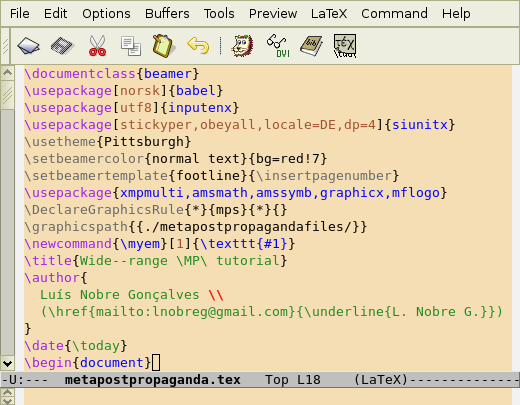
\includegraphics[height=61mm]{metapostpropaganda.png}
  \end{center}
  \href{run:metapostpropaganda.tex}{\underline{See code}}
}

\frame{\frametitle{latexmp}
  \begin{center}
    \includegraphics[height=61mm]{fekslatexmp.1}
  \end{center}
  \href{run:metapostpropagandafiles/fekslatexmp.mp}{\underline{See code}.}  
}

\frame{\frametitle{graphicx}
  \begin{quote}
    \textbackslash usepackage\{graphicx\} \\
    \textbackslash DeclareGraphicsRule\{*\}\{mps\}\{*\}\{\}  \\
    --- \\
    \textbackslash includegraphics[height=61mm]\{fekslatexmp.1\}  
  \end{quote}
}
\frame{\frametitle{beamer+xmpmulti}
  \begin{quote}
    \textbackslash usepackage\{xmpmulti\} \\
    --- \\
    \textbackslash 
      multiinclude[$<+>$][graphics=\{width=8cm\},end=10] \\ 
      \{feksmulti\}
  \end{quote}
}
\frame{\frametitle{GNUPLOT}
  \begin{quote}
    set term mp color solid latex \\
    set output \dq feksgnuplot.mp\dq 
  \end{quote}
}
\frame{\frametitle{xfig}
  \begin{center}
    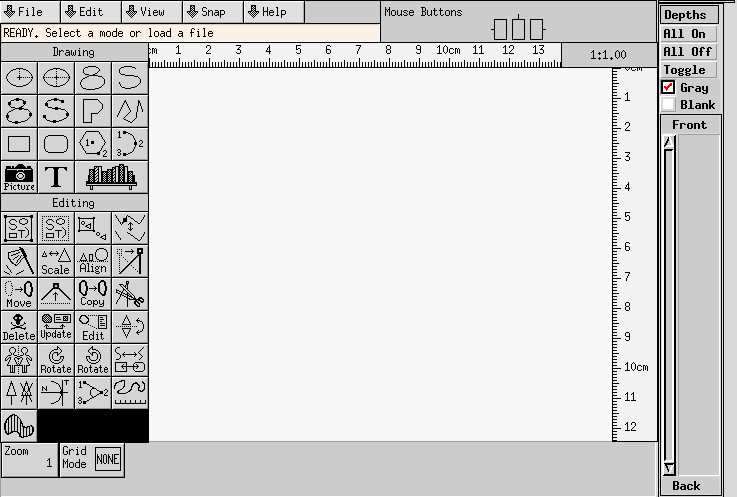
\includegraphics[height=61mm]{xfig.png}
  \end{center}
  fig2ps
}
\frame{\frametitle{dia}
  \begin{center}
    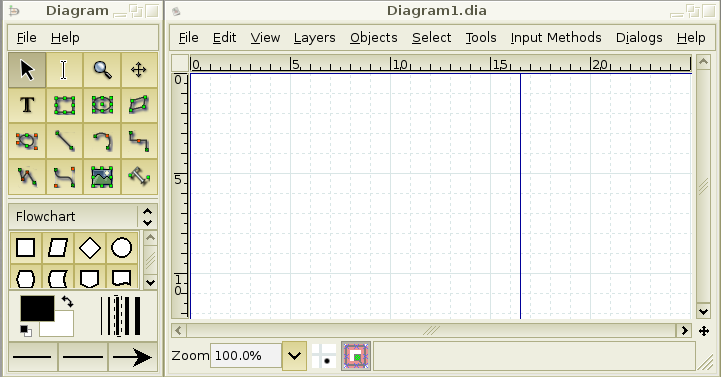
\includegraphics[height=55mm]{dia.png}
  \end{center}
}
\frame{\frametitle{epspdf+gs}
  \begin{flushright}
    epspdf minimal-1.mps \\
    --- \\
    gs -q -sDEVICE=jpeggray -r100 -dNOPAUSE \\
    -sOutputFile=minimal.jpg minimal-1.pdf $<$ /dev/null    
  \end{flushright}
}

\frame{\frametitle{potrace+pstoedit+PstoeditMpostPreeditor}
  \href{http://matagalatlante.org/nobre/MetaPost/debianswirl/DebianSwirl.html}{\underline{Example}}
}

\frame{\frametitle{PstoeditMpostPreeditor}
  \href{http://matagalatlante.org/nobre/MetaPost/QuestionMark/questionmark.html}{\underline{Example}}
}

\section{Workflow}

\frame{
  \frametitle{Basic workflow}
  \begin{center}
    \includegraphics[height=65mm]{workflow-from-mpman-charts.2}
  \end{center}
}

\frame{\frametitle{Workflow}
  \begin{enumerate}
  \item Draw scheme by hand
  \item Identify parameters
    \pause
  \item Express constraints
  \item Determine valid ranges
  \item Program
  \item Test    
  \end{enumerate}
}

\subsection{Workflow example}

\frame{
  \frametitle{Workflow example (0)}
  \begin{center}
    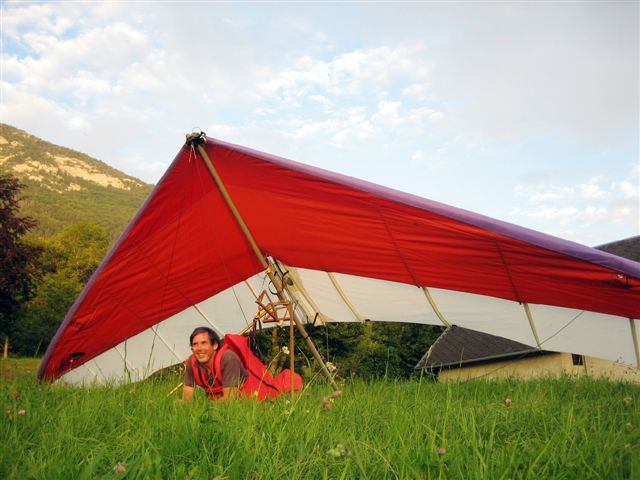
\includegraphics[height=65mm]{pifpafphoto.jpg}
  \end{center}
}

\frame{
  \frametitle{Workflow example (1)}
  \begin{center}
    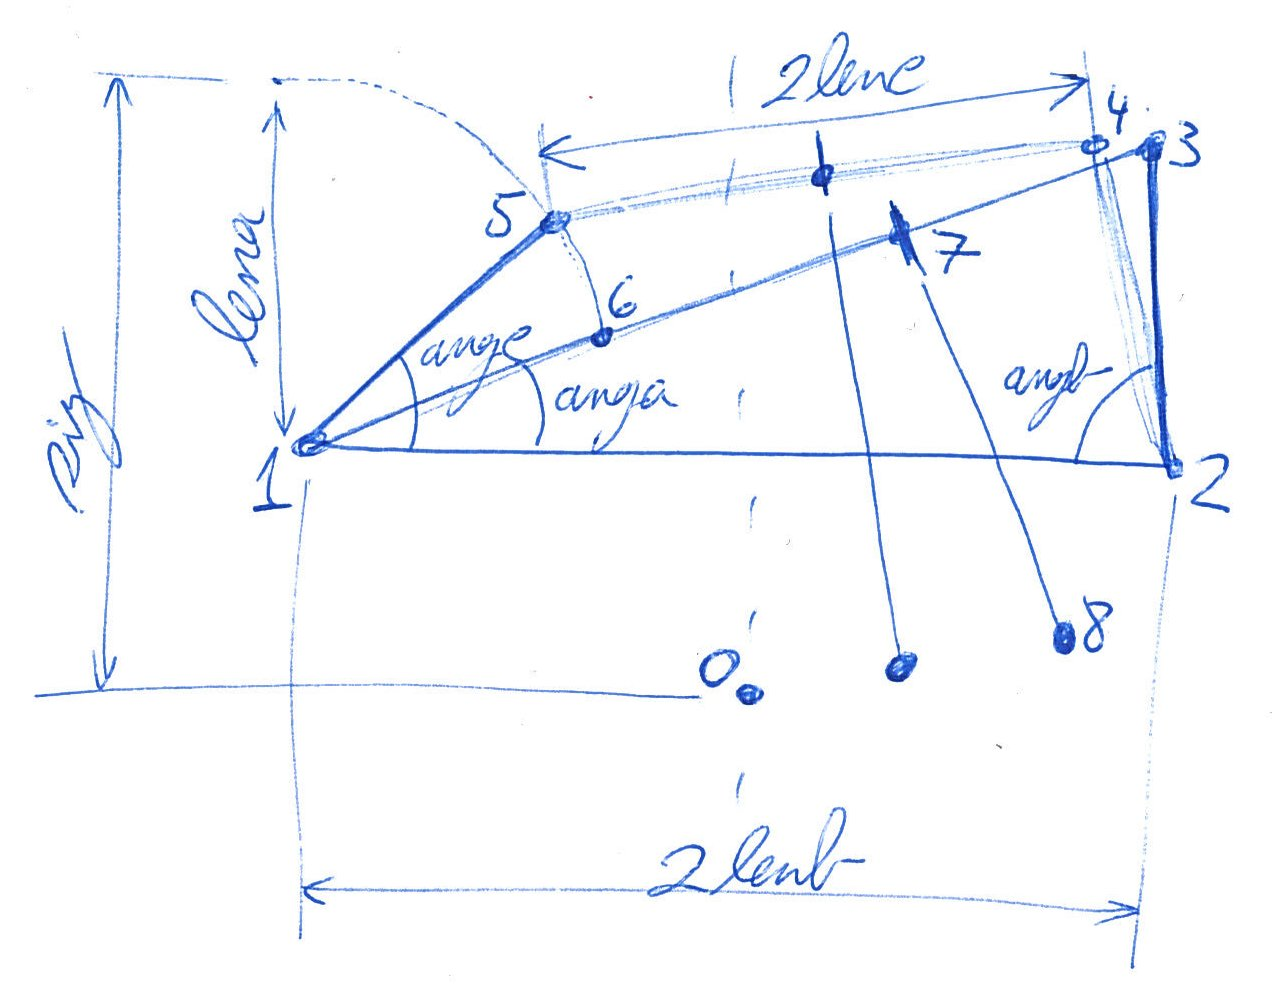
\includegraphics[height=65mm]{pifpaf.jpeg}
  \end{center}
}

\frame{
  \frametitle{Workflow example (2)}
  \multiinclude[<+>][graphics={width=8cm},end=16]{pifpafpropaganda}
}

\end{document}

